\chapter{System Architecture}
\label{chap:5}

\section{Architectural Overview}
\label{sec:5.1}

\begin{figure}[htbp]
\centering
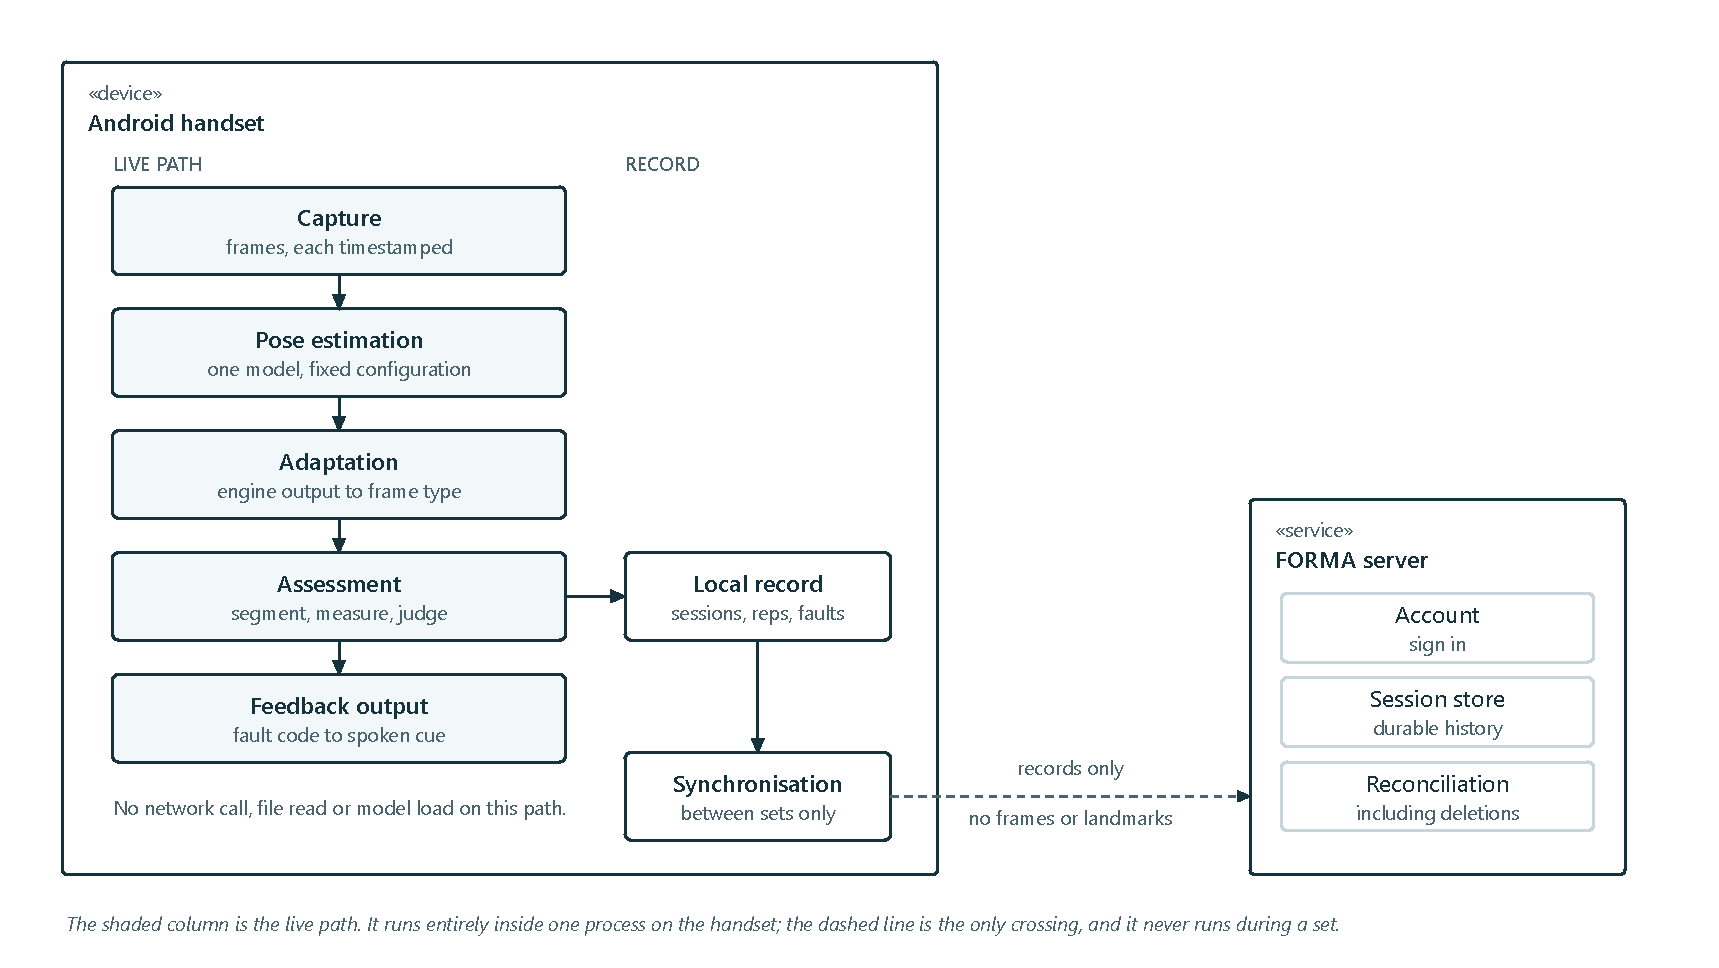
\includegraphics[width=\textwidth]{fig-5-1-architecture.pdf}
\caption[The two deployable parts and the one path with a deadline]{The shaded column is the live path. It runs entirely inside one process on the handset; the dashed line is the only crossing, and it carries records rather than movement.}
\label{fig:5.1}
\end{figure}

The system has two deployable parts and one property worth protecting.

The handset carries the whole of what happens during a set: the camera, the pose model, the assessment layer, and the sound. The server holds the account and the session history. Between them runs a single boundary that is crossed only between sets, and only by derived records.

The property being protected is the one 3.4.1 derives: 300 ms from a fault appearing in the movement to the trainee hearing about it. Everything in the arrangement above follows from refusing to put anything in that path that cannot be bounded. There is no network call on it, no file read, no model load, and no step whose duration depends on anything outside the process.

Two consequences follow, and both are deliberate.

\textbf{A set is complete without a network.} The trainee can train with the phone in aeroplane mode and lose nothing: the count, the faults, the cues and the record are all produced locally. Synchronisation adds durability across devices and is not the price of using the product.

\textbf{The video never exists as a file.} Frames are read from the camera, passed to the model, and released. No frame is written to storage at any point. That makes NFR-S1 a structural claim and not a policy. A reviewer can establish it by reading the code for a write path and finding none.

\section{Layers and Responsibilities}
\label{sec:5.2}

Four layers. Each one is defined as much by what it is forbidden to know as by what it does, because that is what keeps the evaluator testable without a device.

{\small
\setlength{\LTpre}{6pt}\setlength{\LTpost}{8pt}
\begin{longtable}{>{\raggedright\arraybackslash}p{\dimexpr 0.161\textwidth-2\tabcolsep\relax}>{\raggedright\arraybackslash}p{\dimexpr 0.493\textwidth-2\tabcolsep\relax}>{\raggedright\arraybackslash}p{\dimexpr 0.346\textwidth-2\tabcolsep\relax}}
\caption{The layers, what each owns, and what each is not allowed to know}\\
\toprule
Layer & Owns & Must not know \\
\midrule
\endfirsthead
\toprule
Layer & Owns & Must not know \\
\midrule
\endhead
\bottomrule
\endfoot
\bottomrule
\endlastfoot
Perception & Camera frames, the pose model, the output tensor & What an exercise is \\
Adaptation & Model output to the assessment layer's frame type & What the model is \\
Assessment & Segmentation, measurement, verdicts, the trigger policy & That Android exists \\
Presentation & The screen, the spoken cue, the session record & How a verdict was reached \\
\end{longtable}
}

\textbf{Perception has no vocabulary for exercise.} It produces seventeen points with scores, at whatever rate the camera and the delegate allow. It does not know that a squat exists, and swapping the model changes nothing above it.

\textbf{Adaptation is the only layer that knows both sides.} It converts the model's output tensor into the assessment layer's frame type: undoing the letterbox, applying the presence floor, and mapping index to landmark name. 4.2.4 records what this layer costs when it is wrong, which is why it has a layer of its own rather than being folded into either neighbour.

\textbf{Assessment is pure Kotlin with no Android dependency at all.} This is the load-bearing constraint in the whole arrangement. It takes a frame of named landmarks and a timestamp, and returns a phase, a count and a verdict. Because it imports nothing from the platform, a recorded landmark sequence can be replayed through it as an ordinary unit test, which is what makes NFR-A4 checkable and what 10.2 is built on.

\textbf{Presentation owns everything the trainee experiences} and none of the reasoning behind it. It receives a fault code and plays the clip that code names. It cannot compute a verdict and has no access to the geometry, so a change to how a fault is decided cannot reach the interface by accident.

\section{Deployment View}
\label{sec:5.3}

{\footnotesize
\setlength{\LTpre}{6pt}\setlength{\LTpost}{8pt}
\begin{longtable}{>{\raggedright\arraybackslash}p{\dimexpr 0.090\textwidth-2\tabcolsep\relax}>{\raggedright\arraybackslash}p{\dimexpr 0.134\textwidth-2\tabcolsep\relax}>{\raggedright\arraybackslash}p{\dimexpr 0.415\textwidth-2\tabcolsep\relax}>{\raggedright\arraybackslash}p{\dimexpr 0.361\textwidth-2\tabcolsep\relax}}
\caption{Where each part runs, what it holds, and how it is reached}\\
\toprule
 & Runs on & Holds & Reached \\
\midrule
\endfirsthead
\toprule
 & Runs on & Holds & Reached \\
\midrule
\endhead
\bottomrule
\endfoot
\bottomrule
\endlastfoot
Client & The handset & The specifications, the model, the cue bank, the local record & Always \\
Server & A single service & Accounts and the session history & Between sets, when signed in and connected \\
\end{longtable}
}

The client is self-contained. The three specification files, the model and every audio clip ship inside the application bundle, so a first run needs no download and a set can begin seconds after install. Nothing is fetched at runtime.

The server has one job, which 4.3.3 settles: hold the profile and reconcile it with a device that may have been offline for a week. It is deliberately small. It does no pose estimation, no assessment and no scoring, and it never receives an image.

\textbf{What crosses the boundary is the list in FR-22 and nothing else.} Counts, fault codes, timestamps and the specification version in force when the set was performed. The last of those is what lets a record be read correctly later: a fault code means what the specification of that version said it meant, and a record that did not carry its version would become uninterpretable the first time a threshold moved.

\section{Module Structure}
\label{sec:5.4}

Two Gradle modules, and the dependency runs one way.

{\small
\setlength{\LTpre}{6pt}\setlength{\LTpost}{8pt}
\begin{longtable}{>{\raggedright\arraybackslash}p{\dimexpr 0.174\textwidth-2\tabcolsep\relax}>{\raggedright\arraybackslash}p{\dimexpr 0.364\textwidth-2\tabcolsep\relax}>{\raggedright\arraybackslash}p{\dimexpr 0.462\textwidth-2\tabcolsep\relax}}
\caption{The two modules, and the dependency that runs one way between them}\\
\toprule
Module & Depends on & Contains \\
\midrule
\endfirsthead
\toprule
Module & Depends on & Contains \\
\midrule
\endhead
\bottomrule
\endfoot
\bottomrule
\endlastfoot
\texttt{assessment} & kotlinx-serialization only & The specification model, the segmenter, the measurement vocabulary, the evaluator, the trigger policy \\
\texttt{app} & \texttt{assessment}, Android, CameraX, TFLite, Compose & Camera, model, adapter, interface, audio, storage \\
\end{longtable}
}

\textbf{\texttt{assessment} has no Android dependency, and this is enforced rather than intended.} It is a plain Kotlin library. If someone adds an Android import to it, the module stops compiling, so the boundary cannot erode quietly through a convenient import.

Three things follow from it. The assessment layer runs on a desktop JVM, so its tests need no emulator and no device, and they run in seconds as part of an ordinary build. The same code runs unchanged under the offline replay harness in 9.3, which is what allows a recorded video to be scored by exactly the logic that runs on the phone. And the layer most likely to be reused in the second phase is the one with the fewest dependencies.

The module's tests load \textbf{the real specification files} from \texttt{docs/\allowbreak{}specs} rather than copies of them. A specification edited into an invalid state fails the build, which is the only arrangement under which the schema rules stay true of the files that actually ship.

\section{Data Flow}
\label{sec:5.5}

\subsection{The path of one frame}
\label{sec:5.5.1}

\begin{enumerate}
\item \textbf{CameraX delivers a frame} in the analyzer's own thread, with a timestamp taken at capture rather than at arrival.
\item \textbf{The adapter prepares it}: rotate to upright, letterbox into the square the model expects so the aspect ratio survives, hand the buffer over.
\item \textbf{The model returns seventeen keypoints}, each with a score. Points below the presence floor are dropped rather than passed on weak.
\item \textbf{The segmenter updates}: the driver is measured, smoothed, and compared against its hysteresis bounds, producing a phase and, at a boundary, a completed repetition.
\item \textbf{The evaluator judges.} Continuous faults are tested against the frames of their declared phases; per-repetition faults contribute a sample and are decided only at the closing boundary.
\item \textbf{The trigger policy decides whether to speak}, and usually does not.
\item \textbf{A cue plays}, as a clip already in memory.
\end{enumerate}

A frame can leave this path at any of several points, and leaving it is normal. No pose, a landmark below the visibility floor, a phase the fault is not scoped to, a streak too short to confirm, a confidence below the floor, a cue too soon after the last one. Each is a different reason for silence, and 6.5 covers what the trainee is told in each case.

\subsection{A frame that arrives while the engine is busy is dropped}
\label{sec:5.5.2}

The analyzer holds a single flag. If a frame arrives while the previous one is still in the model, the new frame is released immediately and never enters the pipeline.

The alternative is a queue, and a queue is wrong here in a way that gets worse the longer the set runs. Frames arrive at a fixed rate; if the pipeline is slower than that rate for even a short period, a queue grows and every frame in it is older than the movement it describes. The trainee would be corrected about a repetition finished several seconds earlier, and the lag would never recover within the set.

Dropping keeps every frame that is assessed current. The cost is that the effective frame rate is whatever the pipeline can sustain rather than whatever the camera offers, which is exactly the quantity NFR-P2 bounds and 4.2.3 measures.

\subsection{Why the frame rate is a floor rather than a preference}
\label{sec:5.5.3}

A dropped frame is not only a lost measurement. The confirmation window in 3.4.1 is counted in frames, so the frame rate sets how long confirmation takes in wall-clock time.

At 30 fps, three frames of confirmation cost 100 ms. At the 22 fps floor they cost 136 ms. At 15 fps they would cost 200 ms, which is two thirds of the entire response budget spent before the cue is even selected.

This is why frame rate appears in the engine decision twice over, and why 4.2 treats it as reaching further than its own column suggests. Every frame per second buys smoothness in the signal and response time in the cue.

\subsection{What crosses the boundary, and when}
\label{sec:5.5.4}

A set produces one record, written locally when the set ends.

{\small
\setlength{\LTpre}{6pt}\setlength{\LTpost}{8pt}
\begin{longtable}{>{\raggedright\arraybackslash}p{\dimexpr 0.445\textwidth-2\tabcolsep\relax}>{\raggedright\arraybackslash}p{\dimexpr 0.555\textwidth-2\tabcolsep\relax}}
\caption{The fields of a set record, and why each one is kept}\\
\toprule
Field & Why it is kept \\
\midrule
\endfirsthead
\toprule
Field & Why it is kept \\
\midrule
\endhead
\bottomrule
\endfoot
\bottomrule
\endlastfoot
Exercise and specification version & A fault code means what that version said it meant \\
Repetitions, or hold duration & The result the trainee asked for \\
Fault codes with counts & What was detected \\
Per-repetition detail & Which repetitions carried which verdict, and the value behind each \\
Cues spoken & What the trainee actually heard, which is not the same as what was detected \\
Timestamps & Ordering, and the elapsed time of the set \\
\end{longtable}
}

The per-repetition detail is worth its space. A count of faults answers how many; it does not answer which repetitions, or how close the others came to the same verdict. The record stores the value behind every repetition, whether or not it raised anything, so a later reader can tell a repetition that was comfortably correct from one that passed by a hair.

\textbf{Cues spoken is recorded separately from faults raised}, because the two differ by design. The trigger policy suppresses, and a set where six faults were detected and two were spoken is the policy working rather than the detector failing. Reporting only one of the two numbers would hide which.

Synchronisation sends these records and nothing else. No frame, no landmark, and no derived geometry. The server cannot reconstruct the movement from what it holds, which is the point.
